\documentclass{article}


\usepackage{arxiv}

\usepackage{graphicx} %package to manage images

\usepackage[T1]{fontenc}    % use 8-bit T1 fonts
\usepackage{hyperref}       % hyperlinks
\usepackage{url}            % simple URL typesetting
\usepackage{booktabs}       % professional-quality tables
\usepackage{amsfonts}       % blackboard math symbols
\usepackage{amsmath}
\usepackage{nicefrac}       % compact symbols for 1/2, etc.
\usepackage{microtype}      % microtypography
\usepackage{lipsum}
\usepackage{float}
\usepackage{titlesec}
\usepackage[ruled,longend]{algorithm2e}
\usepackage{multicol}


\bibliographystyle{plainnat}

\newcommand{\RNum}[1]{\uppercase\expandafter{\romannumeral #1\relax}}
\titlespacing\section{0pt}{12pt plus 4pt minus 2pt}{0pt plus 2pt minus 2pt}
\titlespacing\subsection{0pt}{12pt plus 4pt minus 2pt}{0pt plus 2pt minus 2pt}
\titlespacing\subsubsection{0pt}{12pt plus 4pt minus 2pt}{0pt plus 2pt minus 2pt}
\graphicspath{ {./images/} }

\title{A Case Study Application in the Performance of Real-time Clouds}


\author{
  Benjamin Bush \\
  Department of Computer Science\\
  Washington University in Saint Louis\\
  Saint Louis, MO 63130 \\
  \texttt{ben.bush@wustl.edu} \\
}

\begin{document}
\maketitle

\begin{abstract}
Despite recent success in generative image modeling, adversarial learning has suffered from producing stable training. In this paper, we empirically investigate the effects of the choice of optimization algorithm and batch size with a deep convolutional AC-GAN on the GAN's training stability and image resolution. Training on the CIFAR-10 dataset, we provide three important recommendations: use Adam as the generator's optimization algorithm, use SGD with Nesterov as the discriminator's optimization algorithm, and use a larger batch size to increase stability of training and resolution of sampled images.  
\end{abstract}
\section{Introduction}
Intelligent Transportation Systems (ITSs) are one of the most anticipated smarty city services and have already seen widespread adoption. The Sydney Coordinated Adaptive Traffic System (SCATS) is a fully adaptive urban traffic control system that optimizes traffic flow and currently operates in more than 37,000 intersections worldwide. Optimizing traffic flow conditions not only shortens travel times, but also can also reduce the carbon emissions generated from road vehicle activity \citep{scats_env}. Unfortunately, city-wide traffic control models are difficult to study using real-world data. While it is possible to develop a model of an ITS using historical data, it is difficult to determine its effectiveness because traffic conditions would morph while under the use of the ITS. Therefore, instead of considering city-wide coordination, this research focuses on the intelligent routing based on real-time prevailing traffic conditions, similar to the service provided by Google Maps. 

Traditional traffic flow models rely on shallow learning algorithms and only a few number of conditions to predict traffic flow. While these models have been moderately successful, they fail to capture the deeper relationship between their features, and also fail to adapt to changing conditions quickly \citep{modeling}. Deep learning methods, on the other hand, have drastically improved the state-of-the-art in a variety of fields such as speech recognition and object detection. Deep learning's success is largely based on its ability to discover intricate structure and relationships between features in large datasets \citep{deep_learning}. The evolution of traffic flow over time is dynamic and non-linear in nature, which makes it a perfect candidate for deep learning methods. With the advent of the Internet of Things (IoT), wireless sensors are able to capture a variety of real world conditions such as traffic accidents, weather, and external events like sports games. ITSs are then able to aggregate these features to build hybrid multimodal methods for traffic flow forecasting using deep learning \citep{hybrid, xiaochus}. 

However, this data transmission and analysis must be performed at ultra-low latency and in real-time in order to have the intended effect of optimizing the operations of a smart city. The combination of compute-intensive workloads and latency-sensitive applications motivates the use of real-time cloud computing. \citep{edge} have recently introduced a framework for efficient edge and cloud computing specifically designed for ITSs, but do not provide empirical results to substantiate their claims. Moreover, current clouds lack service level agreements on latency; these clouds provision resources and not latency. Such a service level agreement is critical for applications like ITSs.

In this paper, we empirically study the latency performance of a simplified ITS on a real-time cloud. The rest of this paper is organized as follows. Section~\RNum{2} presents related work. In Section~\RNum{3}, we provide relevant background information for technologies used. Section ~\RNum{4} covers design and implementation strategies. Section~\RNum{5} presents our empirical study using a real traffic dataset and evaluates the latency of the application on a real-time cloud. Finally, Section~\RNum{6} offers conclusions and directions for future research.
\section{Related Work}
 Traffic flow forecasting has a long history in transportation literature and many kinds of techniques have been proposed to address this problem. \citep{modeling} introduce an autoregressive integrated moving average (ARIMA) process for estimating traffic flows. While the ARIMA model has the benefit that it is easy to interpret, it is not able to accurately capture the non-linear, stochastic nature of traffic flow evolution. \citep{bayesian} have utilized an efficient bayesian particle filter for tracking traffic flows and demonstrated its effectiveness on a dataset from the I-55 highway system in Illinois. The authors then used the same dataset to evaluate a deep neural network with $\ell_{1}$ regularization and applied this model to accurately predict traffic flows during a baseball game \citep{chicago}. \citep{lcrnn} develop a novel model, called LC-RNN, that combines both convolutional and recurrent neural networks in order to more meaningfully learn the time-series and spatio-temporal nature of traffic patterns. 

While deep-learning, specifically time-series-based approaches, have seen the greatest empirical success, it is apparent that no single method works best for every situation.  In general, the most successful methods are hybrid methods that can combine techniques to improve the accuracy of prediction under the prevailing traffic conditions \citep{DBLP:journals/corr/abs-1709-08024}. 
\subsection{Traffic Flow}
Traffic flow forecasting is challenging problem in the space of intelligent traffic management. In this paper, we consider traffic flow in a macroscopic context. That is, instead of considering each vehicle in a traffic stream individually, we rather consider the traffic flow as a measurement at a singled fixed location in space. The traffic flow forecasting problem is thus formally defined as following. At time $T$, we seek to predict the future traffic flow $q_{T+1}$ at time $T+1$ or $q_{T+n}$ at time $T+n$ based on the history of traffic data.

Flow may be considered a temporal measurement and is usually expressed in terms of units over a period of time. For a single lane of traffic, we can define the flow $q$ in region $R$ as
\begin{equation}
    q = \frac{N}{T},
\end{equation}
where $N$ is the number of vehicles observed crossing region $R$ during timespan $T$ \citep{traffic}. For multiple-lane traffic, we can sum the partial flows across each of the $L$ lanes
\begin{equation}
    q = \sum_{l=1}^{L}{q_{l}}  = \frac{1}{T}\sum_{l=1}^{L}{N_{l}},
\end{equation}
where $N_{l}$ is the number of vehicles that passed a detector's site in lane $l$. We also define the mean speed of the traffic stream, expressed in terms of miles (or kilometres) per hour. In this paper, we consider the time-mean speed, which is calculated as the arithmatic average of the vehicles' instantaneous speeds in region $R_{t}$. The time-mean speed is denoted by $\bar{v}_{t}$
\begin{equation}
    \bar{v}_{t} = \frac{1}{N}\sum_{i=1}^{N}{v_{i}},
\end{equation}
where $v_{i}$ is the instantaneous speed of the $i$th vehcile \citep{traffic}.
\subsection{Vanishing Gradient}
The vanishing gradient problem as described in \citep{vangrad} is particularly prevalent in training recursive neural networks. Most neural networks learn weight parameters through some gradient-based optimization method, such as backpropagation through time. For deep or recursive neural networks, backpropagation yields lengthy update equations in which gradients may become vanishingly small, effectively preventing the weight from ever updating its value. There are many methods to combat the vanishing gradient problem in recurrent neural networks, namely the introduction of long short-term memory networks. 
\subsection{Long Short-Term Memory Networks}
Given their capacity to memorize long-term dependencies, long short-term memory (LSTM) neural networks have special advantages for traffic flow prediction. LSTMs are a specific type of recurrent neural network. Recurrent neural networks are comprised of memory cells; memory cells add a loop to the traditional perceptron model of a neural network. These loops make the network recursive, and thereby allow information to persist. Recurrent neural networks have been notable in language modeling, speech-to-text transcript, and other applications with time-series patterns. Whereas traditional recurrent neural networks suffer from the vanishing gradient problem during training, LSTM networks are specifically designed to address the vanishing gradient problem \citep{lstm}. Just like recurrent neural networks, LSTMs are comprised of many memory cells. LSTM networks combat the vanishing gradient problem through the use of forget gates, which are special structures added to the memory cell designed allow the cell to forget certain information. The typical structure of an LSTM memory cell is shown in Figure~\ref{fig:lstm_cell}.
\begin{figure}[ht]
    \centering
    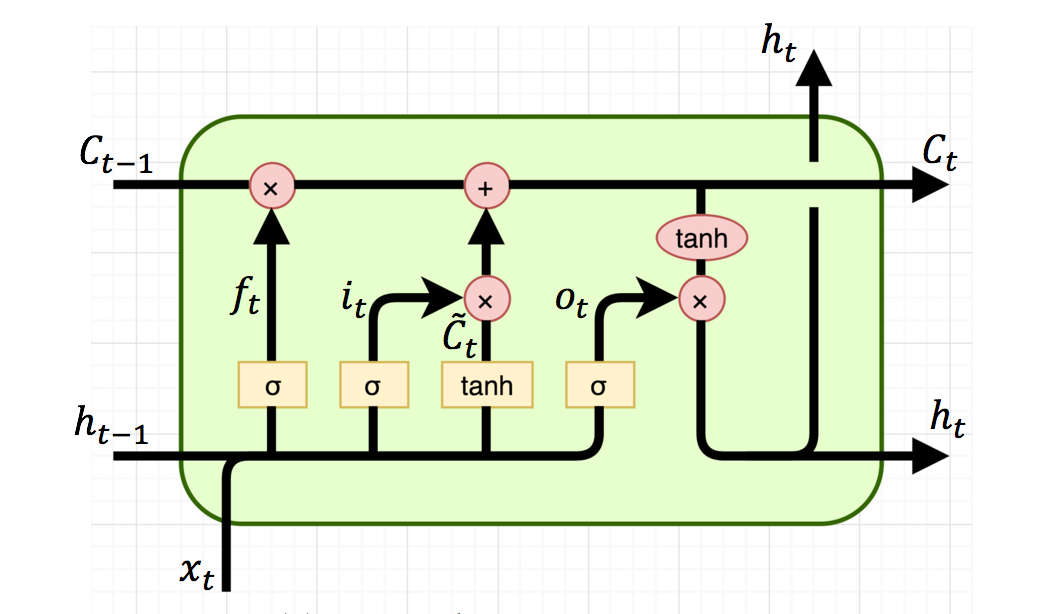
\includegraphics[width=0.8\textwidth]{report/images/lstm_cell2.png}
    \caption{Structure of LSTM memory cell}
    \label{fig:lstm_cell}
\end{figure}


\citep{lstm} describes the information flow for a typical LSTM memory cell-- an LSTM memory cell has three gates: an input gate, a forget gate, and an output gate. Each of these gates are a way to optionally let information through and are comprised of a sigmoid activation function. The sigmoid function squashes values between the range of $[0, 1]$, representing how much information to let through a given gate. At the $t$th timestep, the output from the previous LSTM memory cell, $h_{t-1}$ is fed into the forget gate, which determines how much information from the previous gate to keep, $f_{t}$. The output of the forget gate is then multiplied by the previous cell state. The input gate determines how much information from the most recent observation, $x_{t}$, to include in the cell state. The current cell state, $C_{t}$ is first passed through the $tanh$ activation function, and then multiplied with the output from the input gate, $i_{t}$ , yielding $\Tilde{C}_{t}$. Finally, the current cell state, $C_{t}$ is updated:
\begin{equation}
    C_{t} = f_{t}*C_{t-1} + i_{t}*\Tilde{C}_{t}
\end{equation}
The updated cell state, $C_{t}$ is then fed into the output gate, which determines what the output from the current cell state using the sigmoid function, producing $o_{t}$. The memory cell applies the $tanh$ activation function to the current cell state to squash the values between $[-1,1]$, and multiplies the result with $o_{t}$, producing:
\begin{equation}
    h_{t} = o_{t}*tanh(C_{t})
\end{equation}
While training LSTM networks takes a very long time, stacking many of these LSTM memory cells produces an extremely powerful model capable of learning long-term dependencies, which is particularly useful for predicting traffic flow \citep{xiaochus}. \subsection{A Star Search}
The A Star Search Algorithm ($A^{*}$), is an algorithm used in graph traversal to find the optimal path between any pair of nodes. In our case, we can express a city's roads and freeways as a directed graph in which intersections are nodes and the roads are edges. We can use $A^{*}$ to find the optimal path between any two points in the city. $A^{*}$ is an informed search algorithm that makes use of heuristics to decide which path to consider next. $A^{*}$ determines which path to consider next by minimizing the cost of the current path to the next node, and the estimated cost from the next node to the end. Mathematically, this is expressed as 
\begin{equation}
    f(n) = g(n) + h(n),
\end{equation}
where $g(n)$ is the cost from the start node to node $n$, and $h(n)$ is a heuristic that estimates the cost from node $n$ to the end. In order for $A^{*}$ to be optimal, this heuristic must satisfy two properties: admissibility and consistency. An admissible heuristic is any such heuristic that does not overestimate the true cost of travelling to the next node. A consistent heuristic is any such heuristic that supports the following inequality for any two adjacent nodes, $x$ and $y$
\begin{equation}
    h(x) \leq dist_{x, y} + h(y)
\end{equation}
\section{Background}
This section provides background on the Xen hypervisor, the scheduling framework in Xen. It also describes a stream-processing engine, Flink, and real-time messaging middleware, Kafka.
\subsection{Xen}
Xen \citep{xen} is a popular open-source virtualization platform, which allows multiple virtual machines to share conventional hardware in a safe and resource-managed fashion. Xen serves as a virtual machine monitor (VMM) that lies between the hardware and guest operating systems. Xen controls a special domain, called \textit{domain 0}, which is responsible for managing all other guest domains. Each guest domain acts as a virtual machine (VM), and can specify its resource requirement in terms of the number of virtual CPUs (VCPUs). The typical Xen architecture is shown in Figure~\ref{fig:xen_arch}.  
\textbf{\begin{figure}[ht]
    \centering
    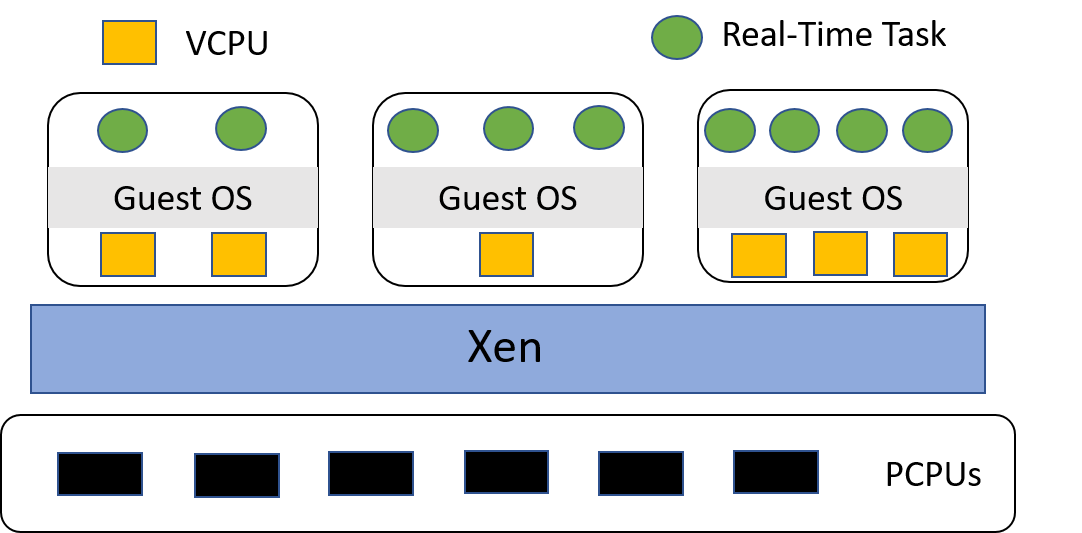
\includegraphics[width=0.4\textwidth]{report/images/xen_arch.png}
    \caption{Architecture of a Xen System}
    \label{fig:xen_arch}
\end{figure}}
Each VM has a guest operating system, which is responsible for scheduling tasks on to VCPUs. Xen is not only responsible for providing virtual resource interfaces to the VMs, but is also responsible for scheduling the VMs onto physical CPUs (PCPUs). There are currently three different schedulers in Xen: Credit, Credit2, and RTDS. Credit is the default scheduler; it is a general purpose weighted fair share scheduler. Credit2 is the evolution of the default Credit scheduler; it is still based on a general purpose, weighted fair share scheme, but is more scalable and efficient with latency-sensitive workloads. RTDS is the real-time deferrable server scheduler that is specifically designed to handle real-time and latency-sensitive workloads \citep{rt-xen}. 
\subsubsection{Credit}
Under the Credit scheduler, each VM specifies a weight and optional cap. The weight corresponds to the share of CPU a VM will have relative to other VMs and the cap encodes the maximum CPU resource a VM can receive. The scheduling algorithm itself is implemented with a partitioned queue: each PCPU maintains a local run queue of VCPUs, sorted by VCPU priority. While a VCPU is scheduled onto a PCPU, it burns credits; once the VM is preempted, VCPU priorities are recalculated based on the weight, cap, and amount of credits consumed. By default, Credit uses a work stealing load-balancing scheme: if a PCPU has no VCPUs in its run queue, it will steal VCPUs from other cores. 
\subsubsection{Credit2}
The Credit2 scheduler is similar to the default Credit scheduler in that it focuses on fairness, but Credit2 also aims to address issues of latency and scalability. Credit2 uses a similar weighting scheme as Credit does by assigning a weight to each VM. Credit2, however, does not have support for caps like Credit does, and is also not CPU mask-aware. As a result, a VM cannot pin its workload to specific PCPUs. 
\subsubsection{RTDS}
Under the RTDS scheduler, each VM specifis a budget and period. While a VCPU is scheduled on to a PCPU, it consumes its budget until the budget is exhausted. The end of the period marks the deadline for a VCPU; at this time, any remaining budget is discarded and then the budget is replenished. The scheduling algorithm is implemented using a global run queue sorted by VCPU deadline. This event-driven approach differs from the quantum-based approach used by the Credit and Credit2 schedulers. As a result, this avoids invoking the scheduler unnecessarily, which should reduce overhead. 
\subsection{Apache Flink}
Apache Flink is a distributed stream-processing engine that provides data distribution, communication, and fault tolerance for distributed computations over data streams. Flink's programing model is a generalization of the MapReduce paradigm. The Flink API offers a set of useful transformation operations, such as join and filter, in addition to the traditional map and reduce functions. Applications specify a series of lazy transformations to an unbounded data stream, which are connected to sources and sinks. The Flink engine then uses a cost optimizer to determine an efficient execution plan called a dataflow. This dataflow is internally represented as a directed acyclic graph from sources to sinks with transformation operators in between. Sinks trigger the execution of the necessary lazy transformations \citep{DBLP:journals/corr/abs-1803-10836}.
\subsection{Apache Kafka}
Apache Kafka is a distributed streaming platform that provides data pipelines and fault tolerance for streams of records across topics. Kafka makes use of two core APIs: the producer API allows an application to publish a stream of record to one or more topics and the consumer API allows an application to subscribe to one or more topics and process the stream of records produced to them. Multiple producers may send streams of records to the same topic and multiple consumers can also subscribe to the same topic. Each topic is spread over a cluster of Kafka brokers, with each broker holding at least one partition of the topic. Kafka uses Apache Zookeeper to help coordinate these services. Kafka is designed to meet high throughput and low latency requirements, making it an extremely suitable choice for real-time streaming applications. 
\section{Design and Implementation}
The previous section provided an overview of background information relevant to the methodology of this paper. This section explores specific design and implementation choices. 
\subsection{Dataset}
In order to create a model of an ITS, we needed historical traffic data to train and test a predictive model as well as data to use to empirically study the latency of the application. The California Transportation Performance Measurement System (PeMS) collects real-time data from nearly 40,000 individual detectors across the freeway system in the state of California. PeMS provides data at a granularity of 5 minute intervals and includes features such as flow and average speed. These features are available across each lane and as aggregates for a given detector station. The raw data that comes from the single lanes is recorded every 30 seconds and then aggregated after every 5 minutes. While the real-time 30 second granularity data is not made publicly available, the 5 minute granularity data is. For this research, we have downloaded data for the month of March 2018 at 5 minute granularity. The data includes the timestamp, flow, and average speed (across individual lanes as well as aggregates); the data were taken from six different detector locations in southern California. Table~\ref{tab:detectors} describes the detector locations and provides their latitude and longitude.  
\begin{table}[ht]
 \caption{Detector Locations}
  \centering
  \begin{tabular}{llllll}
    Detector Number     & Canonical Name & Primary Freeway     & Intersection  & Latitude &  Longitude\\
    \midrule
    1 & El Segundo & 405S   & 105E   & 	33.928621 &	-118.368522\\
    2 & Wilmington & 405S & Wilmington   & 	33.825757 &	-118.24005\\
    3 & Long Beach & 405S & 710S   & 	33.824173 &	-118.207084\\
    4 & Athens & 105E   & 110N   & 	33.928478 &	-118.284031\\
    5 & Lynwood Gardens & 105E & 710S   &	33.914156 &	-118.184451\\
    6 & East Rancho Dominguez & 710S   & East Rancho Dominguez & 	33.877433 &	-118.192776\\


  \end{tabular}
  \label{tab:detectors}
\end{table}
\subsection{Model of ITS}
We seek to create a model of an ITS that will predict future traffic flows and use this prediction to provide optimal routing using the $A^{*}$ algorithm. First, we must create a model that can forecast future traffic flows based on historical data.
\subsubsection{Evaluation Metric}
Given that this is a regression problem, we choose to train our models minimize the mean squared error loss (MSE). MSE is defined as 
\begin{equation}
L = \frac{1}{N}\sum_{i=1}^{N}{(h_{i}-y_{i})^{2}}, 
\end{equation}
where $h_{i}$ is the predicted flow for the $i$th test data point and $y_{i}$ is the true flow. Recall that the MSE loss metric is very sensitive to outliers and noise. To reduce this sensitivity, we preprocess our data by scaling non-time features between the range of 0 and 1. Once the network has been trained and we use it to predict traffic flows, we will transform the prediction back to its original scale. Algorithms 1 and 2 describe how we scale our data down before feeding input into the network, and then transform the data back to its original scale to evaluate the network's performance.
\begin{algorithm}
  $min \gets X.min$\;
  $max \gets X.max$\;
  $X_{scaled} \gets (X - min)/(max - min)$\;
  \KwRet{$X_{scaled}$}\;
  \caption{Preprocess Data}
\end{algorithm}
\begin{algorithm}
  $X_{original} \gets X_{scaled}*(max-min) + min$\;
  \KwRet{$X_{original}$}\;
  \caption{Transform Data to Original Scale}
\end{algorithm}

% so we will also monitor the mean absolute percentage error (MAPE) loss of the models. MAPE is defined as
% \begin{equation}
%     L = \frac{1}{N}(\sum_{i=1}^{N}{\frac{|y_{i}-h_{i}|}{|y_{i}|})}*100\%
% \end{equation}
\subsubsection{Comparison of Methods}
We chose to evaluate five different regression methods and select the model that gave the lowest MSE. We aggregate data across all six detector locations into one cumulative dataset and use this dataset to create a predictor. This cumulative dataset is used to develop our predicted model as well as empirically study the latency o our application on a real-time cloud. We split this dataset into training and testing sets; we used 80\% of the data for training and 20\% of the data for testing. Once the models had been trained, we measured their performance on the unseen test data again using MSE as our metric. Table~\ref{tab:models} presents the MSE (on the original scale) as well as the mean absolute percentage error and $R^{2}$ value for each regressor.
\begin{table}[ht]
 \caption{Model Scores}
  \centering
  \begin{tabular}{llll}
    Model     & MSE & MAPE & $R^{2}$ \\
    \midrule
    LSTM Neural Network & 985.455275 & 23.091062 & 0.962043\\
    Linear Regression & 1013.644990 & 23.702992 & 0.960957\\
    Random Forest & 1083.919621 & 24.140704 & 0.958250\\
    Gradient Boosting Decision Tree & 1151.047555 &25.586357 & 0.955664 \\    
    Decision Tree & 1988.652076 & 32.951715 & 0.923402

  \end{tabular}
  \label{tab:models}
\end{table}
Although all models appear to perform extremely well on our dataset, we choose to select the LSTM neural network for two reasons. First, it is the model that has the lowest score. Second, as we have mentioned in Section~\RNum{2}, LSTM neural networks are the state of the art prediction method for forecasting traffic flows. In order to create the most realistic workload, we should select the model that is most likely to be used in a real world context.  
\subsubsection{LSTM}
We have implemented our LSTM neural network in Python using TensorFlow. Existing studies, such as \citep{deep_learning}, have shown that stacked LSTM layers in a neural network can lead to higher levels of representation of time-series data, which increases the effectiveness of the model. We adopt this architectural choice in the construction of our architecture. In order to prevent overfitting, we utilize dropout-- a technique that randomly drops units and their connections during training \citep{dropout}. The stacked LSTM layers are then connected to two fully connected layers. Recall that we preprocess our data and scale it to a range of 0 and 1, which is why the last layer only has one unit. We use the default activation function for the stacked LSTM layers, $tanh$, but select the rectified linear unit (ReLU) function in our fully connected layers. ReLU is defined as
\begin{equation}
    ReLU(x) = max(0, x)
\end{equation}
ReLU provides two primary benefits. First, it is very easy to compute relative to other activation functions like the sigmoid function or $tanh$, which speeds up training time. Furthermore, ReLU helps prevent the vanishing gradient problem during training. Table~\ref{tab:lstm} summarizes our neural network architecture. 

\begin{table}[ht]
 \caption{LSTM Neural Network Architecture}
  \centering
  \begin{tabular}{lllll}
    Layer & Shape & Dropout & Activation\\
    LSTM & 256 & N/A & tanh\\
    LSTM & 128 & 0.2 & tanh\\
    Dense & 64 & 0.4 & ReLU\\
    Dense & 1 & N/A & ReLU
  \end{tabular}
  \label{tab:lstm}
\end{table}

The network receives a $12$x$1$ vector of scaled traffic flows as input, corresponding to the previous 12 observations of traffic flows, scaled between a range of 0 and 1, at 5 minute intervals. This vector represents the past hour's worth of traffic data. The network predicts the next value of flow, corresponding to traffic flow five minutes in the future. 

We can see from Table~\ref{tab:models} that our trained LSTM neural network performs extremely well on test data. Since the network is trained, we now use it as a predictor in our experiments. 
% * dropout
% * relu activation
% * double stacking the lstm layers
% * glorot uniform initializer
% * why output shape is 1 (scaling/preprocessing)
% * how did we select 12?
\subsubsection{Heuristic}
Recall that we use the traffic prediction as a means of creating a heuristic for our search algorithm. In order for the $A^{*}$ search algorithm to be optimal, the choice of heuristic must be admissible and consistent.

We make use of the average speed measurement as well as our predicted flow in order to create a heuristic function. Consider the case in which we only use predicted flow in our heuristic. A very low prediction for flow might indicative that we expect a lot of heavy, slow moving traffic in which case only a few number of vehicles actually cross the inductor loop. On the other hand, the low value of precited flow might indicate that it is not a busy time on the highway, such as early in the morning. Therefore, we hypothesize that the heuristic would be most informed using information about the predicted flow, and average speed. To enforce admissibility, we bound our heuristic so that it is no greater than the true distance. Because we have the latitude and longitude coordinates, we are able to calculate the true distance along the freeway between any pair of detectors. We therefore define our heuristic as
\begin{equation}
    h(n) = min(0, min(dist_{n}, (70-\bar{v})*q)),
\end{equation}
where $dist_{n}$ is the true distance to node $n$ in the graph, $\bar{v}$ is the average speed across the previous 12 observations, and $q$ is the forecasted flow. Notice that we subtract the average speed from 70, the speed limit on the freeways. This associates a higher cost with very slow moving traffic, and a lower cost for conditions without traffic congestion. Observe that our heuristic is both admissible and consistent by construction, so our $A^{*}$ search algorithm is optimal. 
\subsection{Experimental Setup}
We create two VMs on a server running Xen to handle the dataflow and workload of our experiment. One VM is responsible for producing messages to a Kafka input topic and consuming messages from another Kafka output topic. The other VM is responsible for running a Flink application that will consume messages from the Kafka input topic, pass these records through the pre-trained LSTM neural network to create a prediction, run $A^{*}$ search with this prediction, and then publish results to the Kafka output topic. We denote the former VM as the messaging VM whereas the latter VM is the real-time VM. The messaging VM is responsible for measuring latency, which will be discussed shortly. Figure~\ref{fig:xen_exp_setup} describes the experimental setup. 
\textbf{\begin{figure}[ht]
    \centering
    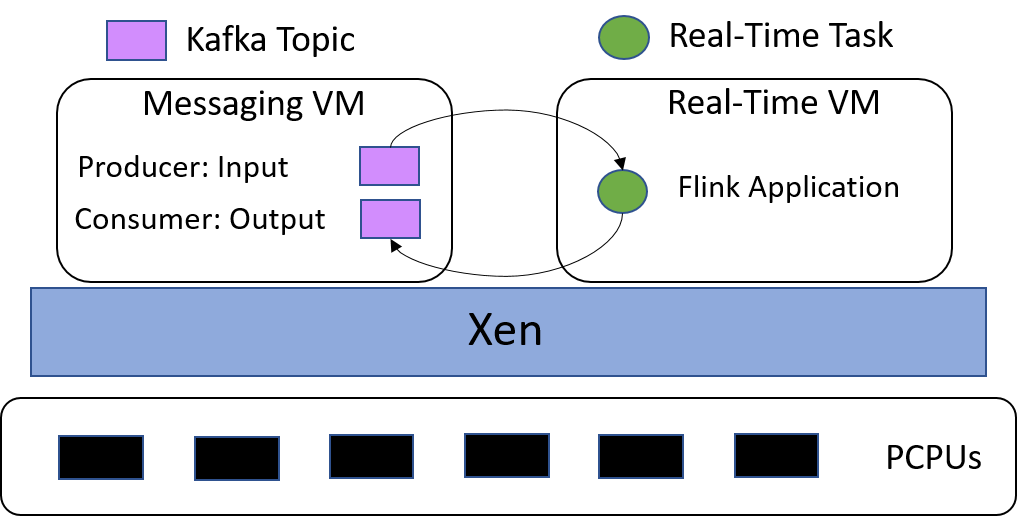
\includegraphics[width=0.5\textwidth]{report/images/xen_exp_setup.png}
    \caption{Experimental Setup}
    \label{fig:xen_exp_setup}
\end{figure}}
\subsubsection{Hardware and Resource Provisioning}
This configuration resides on a server with an 8-core Intel Xeon ES-2620 CPU and 64 GB of memory. The server is configured with Xen 4.10 as the hypervisor and Ubuntu 16.04 as the $domain0$ operating system. Each of the guest domains also run Ubuntu $16.04$.

Within the messaging VM, we created Kafka producers for each detector location for a total of six producers. We created one consumer for the output topic. Recall that Kafka also requires Apache Zookeeper to help coordinate services. Since we want to be able to pin each of these processes to a specific VCPU, the messaging VM requires 8 cores. We allocate 16GB of memory to this machine since it will be responsible for running many services. Within the real-time VM, we will only run the Flink application. We allocate this VM only 2 cores and 8GB of memory.
\subsubsection{Flink Application}
The Flink application provides the workload whose latency we will empirically study. At initialization, the application loads the pre-trained LSTM neural network from memory, and initializes a directed graph. The directed graph consists of nodes representing the detector locations and edges representing the freeways. As a source, the Flink application consumes from the Kafka input topic. Each record contains four fields: a detector location, average speed, traffic flow, and a timestamp. The average speed and traffic flows are both $12$x$1$ vectors of the raw data at 5 minute intervals as captured by the detector. As soon as the application receives a new record, it parses this information and scales the measured flows into the range $[0, 1]$. The application then feeds these scaled flows into the LSTM neural network and creates a prediction, which is immediately transformed back to its original scale. The application then uses this heuristic to run the $A^{*}$ search algorithm to find the optimal path between the El Segundo and Long Beach detectors. Finally, the application creates a new record of the following information: detector location, average speed, traffic flows, timestamp, predicted flow, and path returned by $A^{*}$. As a sink, the Flink application publishes these new records to the Kafka output topic. 
\subsubsection{Latency Calculation}
It is well known that traditional timestamping methods, such as the C routine $dogettimeofday()$, are unrealiable in virtual environments \citep{tsc}. To remedy this issue, we create a custom Python module that utilizes timestamp-counter scaling in order to precisely measure time. This module provides an API to read the current value of the timestamp counter into the edx:eax registers, and return this value. Once we have this value, we can convert it into nanoseconds by dividing by the clock frequency of the CPU, assuming the clock frequency is constant. To enforce a constant clock frequency, we change the power settings in the system's BIOS. Although the CPU can optimize its power consumption through different p-states (performance states), and minimize power consumption through c-states, these create variability in the clock frequency of the CPU. By disabling these features, we fix the clock frequency. In our case, we fixed the clock frequency to 2.1GHz. We implement highly precise latency calculations in the messaging VM using this method. 

Each producer makes a call to the custom module just before sending the message and appends the nanosecond timestamp to the record. When the consumer receives a record, it has access to this original timestamp. Therefore, the consumer can make a call to the custom module and timestamp as soon as it receives a new record; the difference between these two timestamps represents the latency of the application in nanoseconds.
\section{Evaluation}
We empirically evaluate the latency of the Flink application on each of the three schedulers within Xen. One experiment corresponds to sending 20,000 records through the Flink application and recording the latencies for a given configuration. Each of the six producers sends a message from their detector location once every 100ms. Although real-world data come only every 5 minutes, we accelerate the rate in order to achieve a suitable workload.  
\subsection{RTDS}
Recall that within the RTDS scheduler, each VM must specify a budget and a period. Given that producers are sending messages once every 100ms, we set the period of the real-time VM to 100ms. Initially, we provide the real-time VM with access to the entire PCPU -- that is we set the budget equal to the period of 100ms. An ECDF curve of this configuration is shown in Figure~\ref{fig:rtds_full}.
\textbf{\begin{figure}[ht]
    \centering
    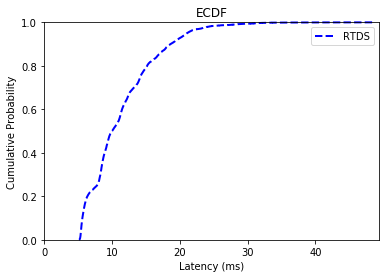
\includegraphics[width=0.4\textwidth]{report/images/rtds_full.png}
    \caption{ECDF of Latency Distribution RTDS Scheduler}
    \label{fig:rtds_full}
\end{figure}}
We can also specify a budget less than the value of the period, effectively giving the real-time VM partial access to the CPU, or a "partial-CPU." The benefit of the not consuming the entire period is that the system may reclaim idle clock cycles and improve overall efficiency. If we keep the period the same, then we can discover a budget that gives the same latency performance as if the real-time VM had exclusive access to the CPU. We do so by first allocating a very small budget, and then inrementally increasing the budget until the ECDF curves overlap. In nearly all cases the the budget was smaller than the period, the maximum latency of the partial-CPU experiments were greater than those of the full-CPU counterpart. Table~\ref{tab:rtds} summarizes these results.
\begin{table}[ht]
 \caption{Maximum Latencies for RTDS Experiments}
  \centering
  \begin{tabular}{llll}
    Scheduler & Budget ($\mu$s) & Period ($\mu$s) & Maximum Latency (ms)\\
    RTDS & 100000 & 100000 & 48.52186857142857\\
    RTDS & 80000 & 100000 & 55.77778047619047\\
    RTDS & 77500 & 100000& 38.0649180952381\\
    RTDS & 76750 & 100000& 49.31550476190476 \\
    RTDS & 76000 & 100000& 61.50309523809524 \\
    RTDS & 75000 & 100000& 55.69025428571428
  \end{tabular}
  \label{tab:rtds}
\end{table}
When we set the budget to 777500, we actually observe an improvement in the maximum latency observed. On the other hand, almost all of the partial-CPU experiments yielded ECDF curves that indicated a critical majority of the latencies were smaller than those of the full-CPU counterparts. Consider Figure~\ref{fig:rtds_77500}, which shows the ECDF curves of the full-CPU and budget=77500 experiments. 
\textbf{\begin{figure}[ht]
    \centering
    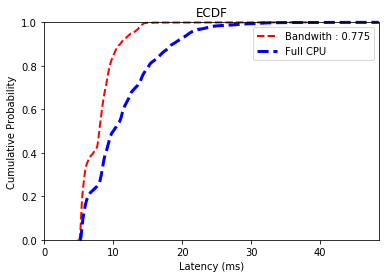
\includegraphics[width=0.4\textwidth]{report/images/rtds_77500_100000.png}
    \caption{ECDF Latency Distribution Partial CPU (0.775) vs. Full CPU RTDS Scheduler}
    \label{fig:rtds_77500}
\end{figure}}

Not only does this experiment have a smaller maximum latency, and therefore can provide a better service-level agreement, but the ECDF curve also lies above that of the full-CPU experiment. This behavior is also exhibited in the other experiments with budgets greater than 76750. The experiment with budget set to 76750 showed near equivalent performance both in terms of maximum latency, as seen in Table~\ref{tab:rtds}, but also with respect to their ECDF curves as seen in Figure~\ref{fig:rtds_76750}.
\textbf{\begin{figure}[ht]
    \centering
    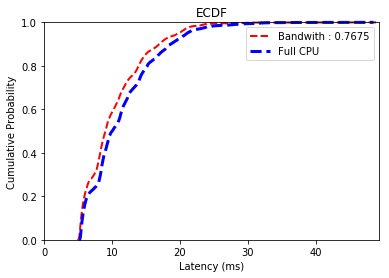
\includegraphics[width=0.4\textwidth]{report/images/rtds_76750_100000.png}
    \caption{ECDF Latency Distribution Partial CPU (0.7675) vs. Full CPU RTDS Scheduler}
    \label{fig:rtds_76750}
\end{figure}}
\subsection{Credit}
Under the default Credit scheduler, each VM can specify a weight and optional cap. The cap is expressed in terms of the number of VCPUs. While it is not a direct equivalence, we can vary the cap parameter for the real-time VM to achieve a similar effect as the partial-CPU cases that were discussed with RTDS above. We therefore conduct two experiments: one without any caps, and one with a cap. Recall that the partial-CPU experiment that was most similar to the full-CPU experiment using the RTDS scheduler had a budget of 76750 and a period of 100000. Therefore, since the real-time VM had 2 cores, it effectively made us of $\frac{76750}{100000}*2 = 153\%$ of a single PCPU. Because the cap parameter in Credit is expressed in terms of percentage of CPUs, we set the cap of the real-time VM to be 153 for the partial-CPU Credit experiment. Table~\ref{tab:credit} summarizes the experimental results. 
\begin{table}[ht]
 \caption{Maximum Latencies for Credit Experiments}
  \centering
  \begin{tabular}{lll}
    Scheduler & Cap & Maximum Latency (ms)\\
    Credit & 0 (None) & 116.94941476190476\\
    Credit & 153 & 1040.939347142857
  \end{tabular}
  \label{tab:credit}
\end{table}

Figure ~\ref{fig:credit_full} shows the ECDF curves for the full CPU experiments using Credit and RTDS schedulers. 
\textbf{\begin{figure}[ht]
    \centering
    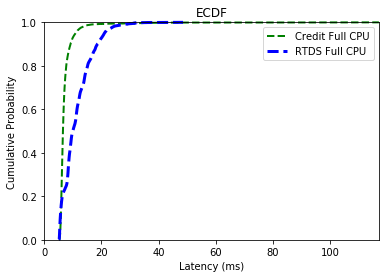
\includegraphics[width=0.4\textwidth]{report/images/credit_full.png}
    \caption{ECDF Latency Distribution Full CPU Credit vs. Full CPU RTDS}
    \label{fig:credit_full}
\end{figure}}
The full-CPU Credit scheduler distribution exhibits similar characteristics to the partial-CPU RTDS experiments. The majority of the Credit ECDF curve lies above that of the RTDS and it has a higher maximum latency. Figure~\ref{fig:credit_partial} shows the ECDF curves for the partial CPU experiments using Credit and RTDS schedulers. 
\textbf{\begin{figure}[ht]
    \centering
    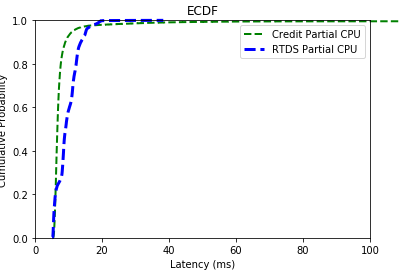
\includegraphics[width=0.4\textwidth]{report/images/credit_partial.png}
    \caption{ECDF Latency Distribution Partial CPU Credit vs. Partial CPU RTDS}
    \label{fig:credit_partial}
\end{figure}}
Observe that the green line corresponding to the Credit Partial CPU ECDF curve trails off of the plot. This is because the maximum latency of the partial-CPU credit experiment was abysmally large-- over a second. If the plot were to show the entire graph, the two curves would be indistinguishable, so we limit the X-axis for readibility. 
\subsection{Credit2}
Although Credit2 is the evolution of the Credit scheduler, it does not yet support a cap feature. As a result, we cannot run experiments that limit the CPU of a VM. We therefore only run one experiment, equivalent to the full-CPU scenarios described above. Table~\ref{tab:credit2} summarizes the experimental results. 
\begin{table}[H]
 \caption{Maximum Latencies for Credi2t Experiments}
  \centering
  \begin{tabular}{ll}
    Scheduler & Maximum Latency (ms)\\
    Credit2 & 951.1479685714286\\
  \end{tabular}
  \label{tab:credit2}
\end{table}
Credit2 suffered from the same behavior that was observed under the default credit scheduler-- the maximum latency was tremendously large even though a significant portion of the records were processed faster than in RTDS. Figure~\ref{fig:credit2_all} shows the ECDF curves for all three full-CPU experiments.
\textbf{\begin{figure}[ht]
    \centering
    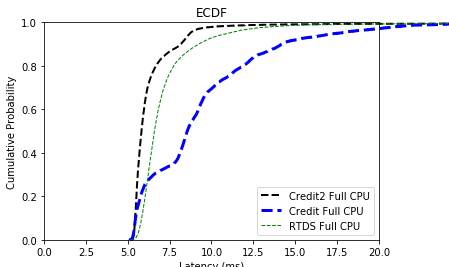
\includegraphics[width=0.4\textwidth]{report/images/credit2_all.png}
    \caption{ECDF Latency Distribution Full CPU Credit2 vs. Full CPU Credit vs. Full CPU RTDS}
    \label{fig:credit2_all}
\end{figure}}
Observe that we limited the X-axis of this plot for readability due to the same reasons discussed above: the large maximum latency would otherwise make the graphs indistinguishable. 


It is readily apparent that the choice of hypervisor is largely dependent on the use case. For applications that require ultra low-latency service level agreements, the RTDS scheduler is the clear choice. For other applications that are more concerned with median performance, then the Credit and Credit2 schedulers seem to provide better performance. Although we artificially accelerated the input rate of the producers to achieve a more critical workload, this workload demonstrates the performance benefits and drawbacks of each scheduler. 
\section{Conclusion}
We have developed a model of an ITS that provides real-time optimal routing through the use of traffic forecasting. We have used this model as workload to empirically study the effect the choice of scheduler has on the latency of the application. It is evident from these experiments that the choice of scheduler largely depends on the use case of the application. The RTDS scheduler provides excellent latency guarantees whereas the Credit and Credit2 schedulers are more general-purpose. It is important to note that we have sacrificed a few real-world conditions in order to create a viable workload. First, we have statically defined the start and end locations for our $A^{*}$ search algorithm, whereas in the real world they would certainly be more dynamic and would the network graph would be significantly larger in order to accurately represent the roads and freeways of the surrounding area. Additionally, we have artificially increased the rate of input in order to achieve a critical workload to demonstrate the effectiveness of the three schedulers. Although most cities do not currently have real-time traffic data, the advent of self-driving cars and other IoT devices has significant implications for the amount of data being transmitted and computed. This work creates several future research opportunities in a variety of different areas. It may be useful to examine source code to better understand why the RTDS scheduler lacks some aspects of efficiency relative to Credit and Credit2. This work may also be extended in order to compare the effects of different architecture choices such as the choice of a different messaging middleware. Lastly, although this work provides a basic model of an ITS with routing capabilities, there are many possible features to integrate into this model to make it more applicable to the real world. 
\bibliographystyle{unsrt}
\bibliography{references}

\end{document}